%.-------------------------------------------------------------------------------------------------------------------------------------------------------------

The System is divided in various subsystems:
\begin{itemize}
\item Mobile App
\item Web Application
\item Web Server
\item Application Server
\item DataBase Connection
\item DataBase Server 
\item External Systems:Google Maps,External DataBases
\end{itemize}
The subsystems not external will be implemented and tested. They will also be integrated together, and with external systems. Since the Web Server provides user only static data (HTML, CSS, JavaScript) and is deployed to a different device than the web Application, this component can be implemented and tested in any moment during the development but the integration must be done when the full application is implemented. Given our design choice of having a multiple servlet server which communicates with DataBase through a facade, our implementation must have as a starting point the implementation of the DataBase Server and the connection with it.
%----------------------------------------------------------------------------------------------------------------------------------------------------------------------------------------------------------------------------------------------
\subsection{DataBase Server and Connection}
\begin{figure}[H]
\centering
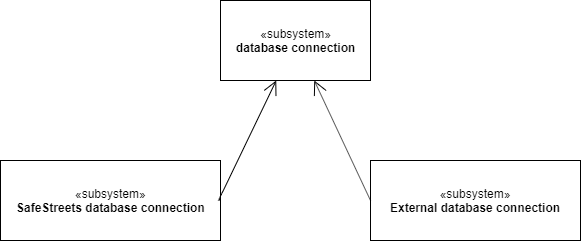
\includegraphics[width=\textwidth]{Images/TestDBdiagram.png}
\caption{\label{fig:ComWI}Database Server and Connection Integration}
\end{figure}
This phase is important so several test will be run to check the correct functioning of the connection
and the functions for data access needed by the system. In this phase also the abstract classes
for the connection to external DataBases will be implemented and tested with a dummy DataBase to test
that the design choice for external DataBase works correctly. Then the DataBase connection is implemented and integrated with the DataBase Server and the External DataBase connection subsystems. The testing phase must cover as much cases as possible and different test approaches must be used to test
the functionalities provided by DataBase Connection subsystem. After this initial phase the Application
Server must be implemented

%----------------------------------------------------------------------------------------------------------------------------------------------------------------------------------------------------------------------------------------------
\subsection{Web Application}
\begin{figure}[H]
\centering
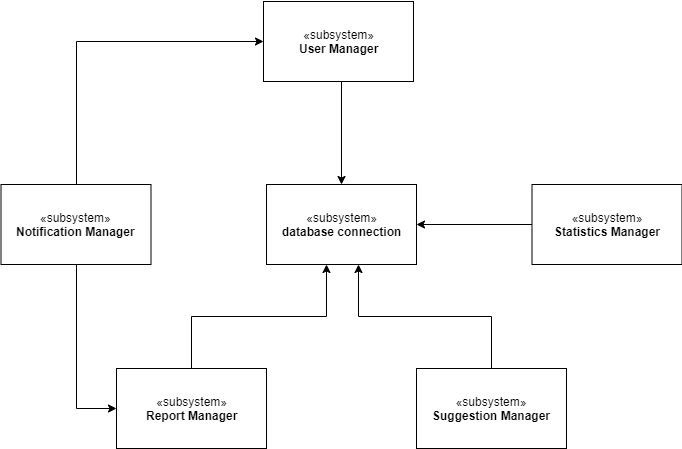
\includegraphics[width=\textwidth]{Images/TestServlet.png}
\caption{\label{fig:ComWI}Servlet Integration}
\end{figure}
The implementation and testing can be performed in parallel for all the managers except for the Notification Manager which requires the implementation of the Report Manager and of the User Manager. All these components must be tested using test stubs to access and test functionalities of the managers, covering all of them and using coverage tests to check if all the checks done on data, and all possible kind of issues (I.e. missing DataBase, null values, exceptions) are handled and there are no controls which aren’t reachable for any kind of input. The components are then integrated with the DataBase Connection subsystem
%----------------------------------------------------------------------------------------------------------------------------------------------------------------------------------------------------------------------------------------------
\subsection{Mobile App and Web Application}
\begin{figure}[H]
\centering
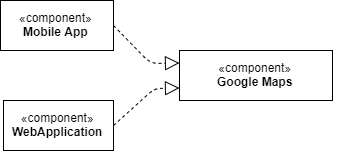
\includegraphics{Images/IntegrationMaps.png}
\caption{\label{fig:ComWI}Google Maps Integration}
\end{figure}
In parallel to the implementation of Application Server the development of the WebApplication and
Mobile App can be carried on.

\begin{figure}[H]
\centering
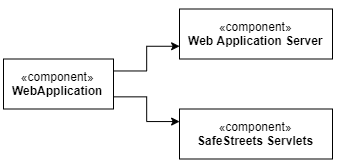
\includegraphics{Images/IntegrationWeb.png}
\caption{\label{fig:ComWI}Web Application Integration}
\end{figure}
After the implementation both needs to be integrated with APIs provided by Google Maps and when
Application Server development will be complete they will be integrated and tested together. Web Application also needs to be integrated and tested with Web Server.

\begin{figure}[H]
\centering
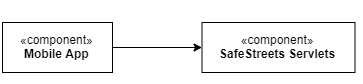
\includegraphics{Images/IntegrationMobile.png}
\caption{\label{fig:ComWI}Mobile Applicaiton Integration}
\end{figure}
%----------------------------------------------------------------------------------------------------------------------------------------------------------------------------------------------------------------------------------------------
\newpage
\subsection{Main feature test plan after all components are integrated}
Once all the systems are integrated an additional testing phase will be devoted to check the possible interaction of users with the system. For the main functionalities and interactions in the mobile application
testing we will use some flowcharts, and do coverage testing over them and check that no unexpected results occurs with different values when citizens make reports, and when authorities accepts and terminate assignments.

\begin{figure}[H]
\centering
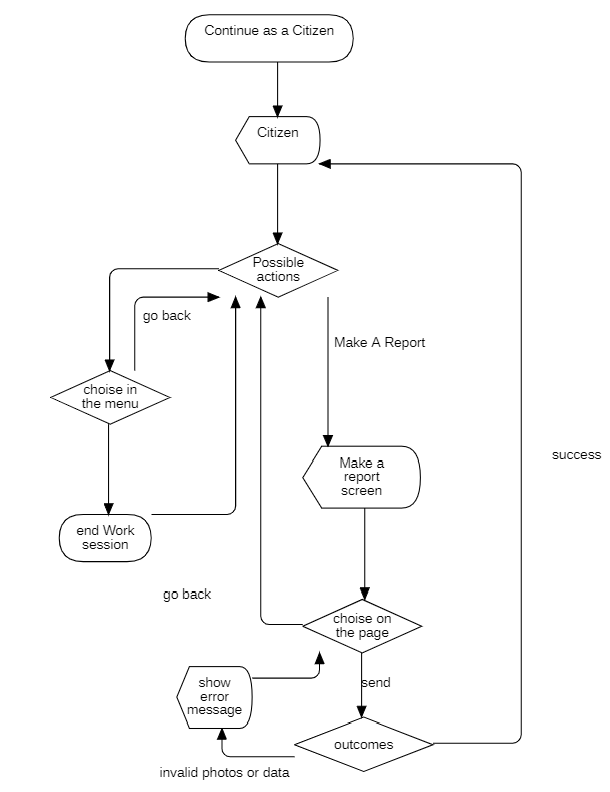
\includegraphics{Images/FlowChartCitizen.png}
\caption{\label{fig:ComWI}FlowChart: Citizen main features testing}
\end{figure}
\newpage
\begin{figure}[H]
\centering
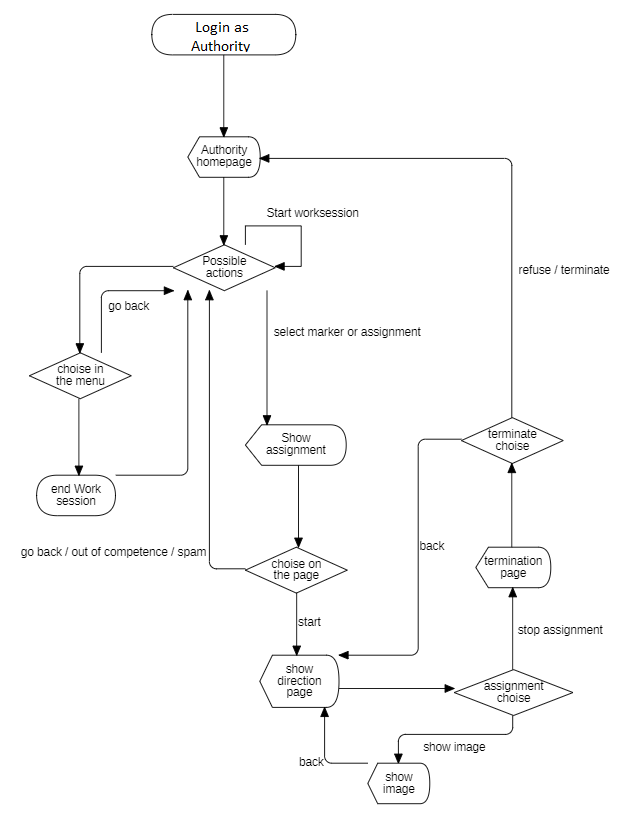
\includegraphics{Images/FlowChartAuthority.png}
\caption{\label{fig:ComWI}FlowChart: Authority main features testing}
\end{figure}


